%
% This presentation is for use at the MDACC Medical Physics Trainee 2015 Summer
% Seminar Series on July 6, 2015.
%

\documentclass{beamer}
\usepackage{amsmath}
\usepackage{graphicx}
\usetheme{Warsaw}
\graphicspath{{Images/}}

%%%%%%%%%%%%%%%%%%%%%%%%%%%%%%%%%%%%%%%%%%%%%%%%%%%%%%%%%%%%%%%%%%%%%%%%%%%
% Title Page
%%%%%%%%%%%%%%%%%%%%%%%%%%%%%%%%%%%%%%%%%%%%%%%%%%%%%%%%%%%%%%%%%%%%%%%%%%%
\title[Spinal Cord DWI with Reduced FOV ss-EPI]{DWI of the Spinal Cord with Reduced FOV Single-Shot EPI}
\author{Drew Mitchell}
\institute{MD Anderson Cancer Center}
\date{June 17, 2015}
%\AtBeginSection[]
%{{
%\setbeamertemplate{headline}{}
%\frame{\tableofcontents[currentsection]}
%}}

\begin{document} 
{
\setbeamertemplate{headline}{}
\frame{\titlepage}
\frame{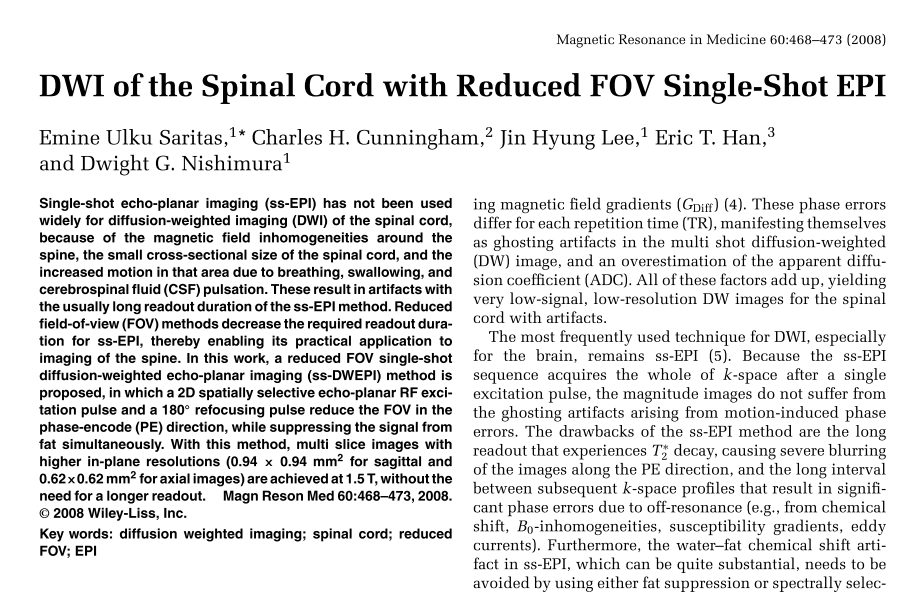
\includegraphics[height=7cm]{SpineDWI}}
\begin{frame}{Table of Contents}
\tableofcontents
\end{frame}
}

%%%%%%%%%%%%%%%%%%%%%%%%%%%%%%%%%%%%%%%%%%%%%%%%%%%%%%%%%%%%%%%%%%%%%%%%%%%
% Introduction
%%%%%%%%%%%%%%%%%%%%%%%%%%%%%%%%%%%%%%%%%%%%%%%%%%%%%%%%%%%%%%%%%%%%%%%%%%%
\section{Introduction}

\begin{frame}{Introduction}
\begin{itemize}
	\item Spinal cord diffusion-weighted imaging (DWI) can diagnose disorders from fiber tract damage
	\item Several challenges:
	\begin{itemize}
		\item Magnetic field inhomogeneities around spine create off-resonance artifacts
		\item Partial volume effects from CSF and lipid
		\item Spinal cord cross section very small
		\item Bulk physiologic motion from heart, breathing, swallowing, CSF pulsation
	\end{itemize}
	\item Phase errors differ for each TR, make ghosting artifacts for multi shot DWI, and overestimate apparent diffusion coefficient (ADC)
	\item Result is low-signal, low-resolution DW images with artifacts in spinal cord
\end{itemize}
\end{frame}

\begin{frame}{Introduction}
\begin{itemize}
	\item Single-shot echo planar imaging (ss-EPI) most frequently used technique for DWI
	\item Advantages:
	\begin{itemize}
		\item Acquires whole k-space after single excitation pulse
		\item No ghosting artifacts from motion-induced phase errors
	\end{itemize}
	\item Drawbacks:
	\begin{itemize}
		\item Long readout experiences $T_2^*$ decay, blurring images in PE direction
		\item Long interval between k-space profiles result in phase errors from off-resonances
		\item Water-fat chemical shift artifacts are severe and must be avoided by fat suppression or spectrally selective excitation
	\end{itemize}
	\item Magnetic field inhomogeneities around the spine, plus these drawbacks, make quality ss-EPI spinal cord images difficult
\end{itemize}
\end{frame}

\begin{frame}{Introduction}
\begin{itemize}
	\item Spinal cord imaging benefits from reduced FOV applications (because of narrow anatomy)
	\item Reduced FOV methods decrease the readout duration, reduce off-resonance artifacts, and enable ss-EPI techniques
	\item Excited FOV in PE direction reduced by using 2D spatially selective echo-planar RF excitation pulse and $180^{\circ}$ refocusing RF pulse
	\item Required number of k-space lines in PE direction decreased by reducing FOV, which leads to higher resolution for fixed scan time
	\item Combination of 2D RF pulse and $180^{\circ}$ refocusing RF pulse allows multi slice imaging and suppresses fat signal
\end{itemize}
\end{frame}
	
%%%%%%%%%%%%%%%%%%%%%%%%%%%%%%%%%%%%%%%%%%%%%%%%%%%%%%%%%%%%%%%%%%%%%%%%%%%
% Theory
%%%%%%%%%%%%%%%%%%%%%%%%%%%%%%%%%%%%%%%%%%%%%%%%%%%%%%%%%%%%%%%%%%%%%%%%%%%
\section{Theory}

\begin{frame}{Theory}
\begin{columns}[T]
	\begin{column}[T]{5cm}
		In this paper, a standard DW spin-echo ss-EPI sequence is used, with excitation pulse replaced with $90^{\circ}$ 2D spatially selective echo-planar RF pulse that reduces FOV in PE direction
	\end{column}
	\begin{column}[T]{5cm}
		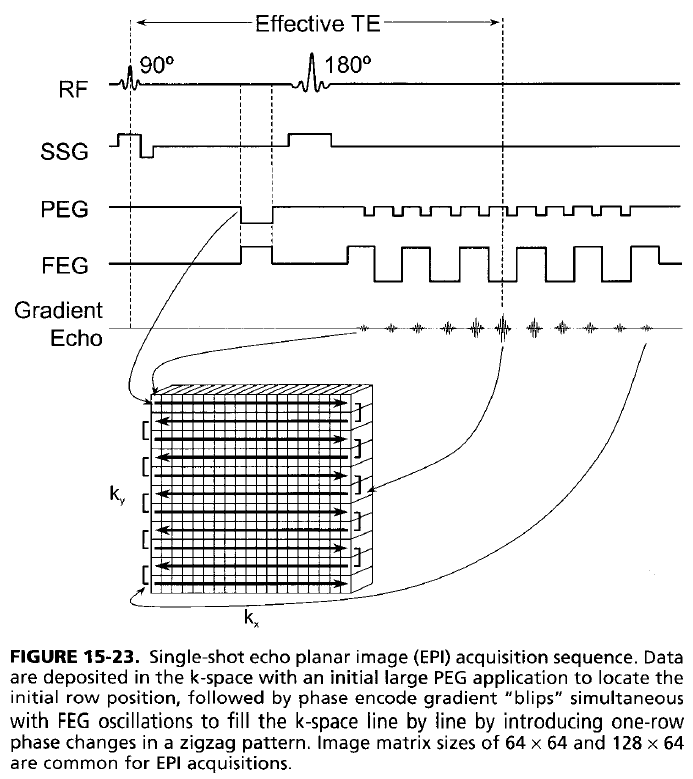
\includegraphics[height=6cm]{BushbergEPI}
	\end{column}
\end{columns}
\end{frame}

\subsection{2D Echo-Planar RF Pulse}

\begin{frame}{2D Echo-Planar RF Pulse}
\begin{columns}[T]
	\begin{column}[T]{5cm}
		\begin{itemize}
			\item 2D echo-planar pulses provide control of slice thickness in two orthogonal directions independently by combining two RF pulses
			\item The "slow" (blipped) and the "fast" axes gradients and RF pulses are designed to achieve desired excitation profiles in each spatial direction for EPI trajectory through k-space
		\end{itemize}
	\end{column}
	\begin{column}[T]{5cm}
		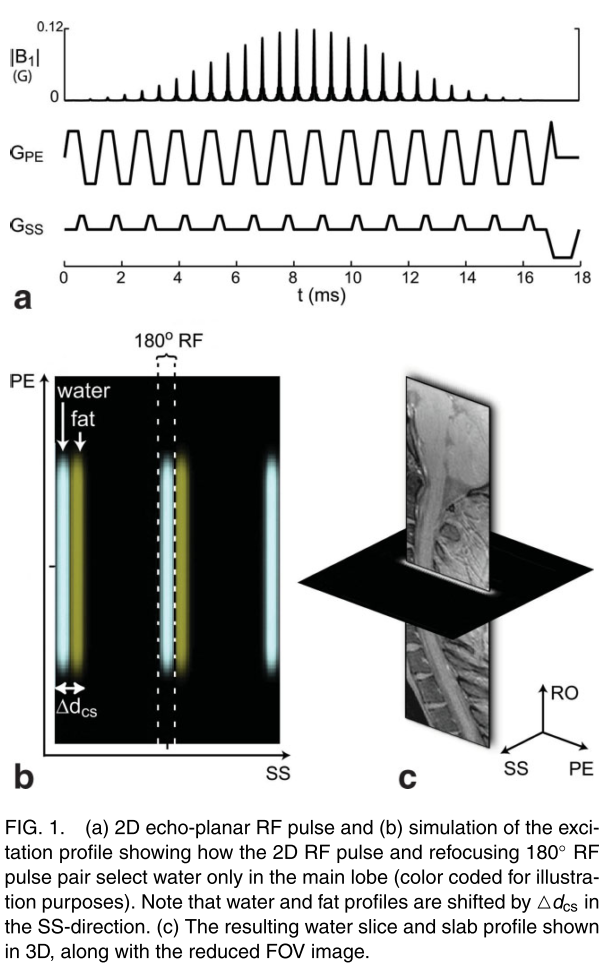
\includegraphics[height=6cm]{SpineDWIfig1}
	\end{column}
\end{columns}
\end{frame}

\begin{frame}{2D Echo-Planar RF Pulse}
\begin{columns}[T]
	\begin{column}[T]{5cm}
		\begin{itemize}
			\item The two orthogonal directions are the slice-select (SS) direction and the slab-select direction (phase encode direction during imaging)
			\item The echo-planar RF pulse creates a $90^{\circ}$ flip angle over 4 mm (SS direction) $\times$ 4.5 cm (PE direction) slab
		\end{itemize}
	\end{column}
	\begin{column}[T]{5cm}
		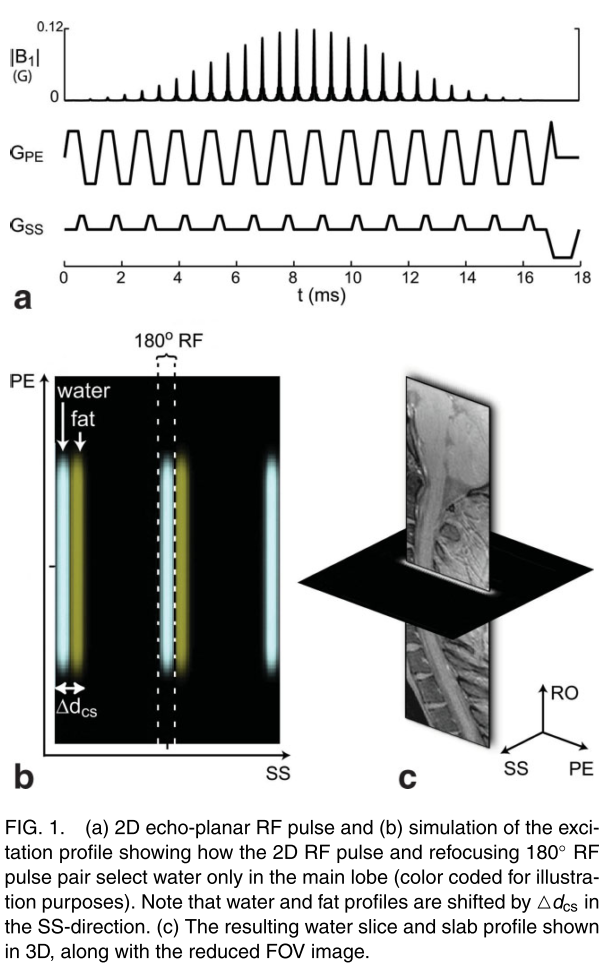
\includegraphics[height=6cm]{SpineDWIfig1}
	\end{column}
\end{columns}
\end{frame}

\begin{frame}{2D Echo-Planar RF Pulse}
\begin{columns}[T]
	\begin{column}[T]{5cm}
		\begin{itemize}
			\item The pulse duration is 16.8 ms with 14 blips in the SS direction
			\item The excitation profiles for fat and water are displaced in volume along the blipped (SS) direction
			\item Excitation profile period in SS direction, because blipped gradients in SS direction fill RF excitation k-space discretely
		\end{itemize}
	\end{column}
	\begin{column}[T]{5cm}
		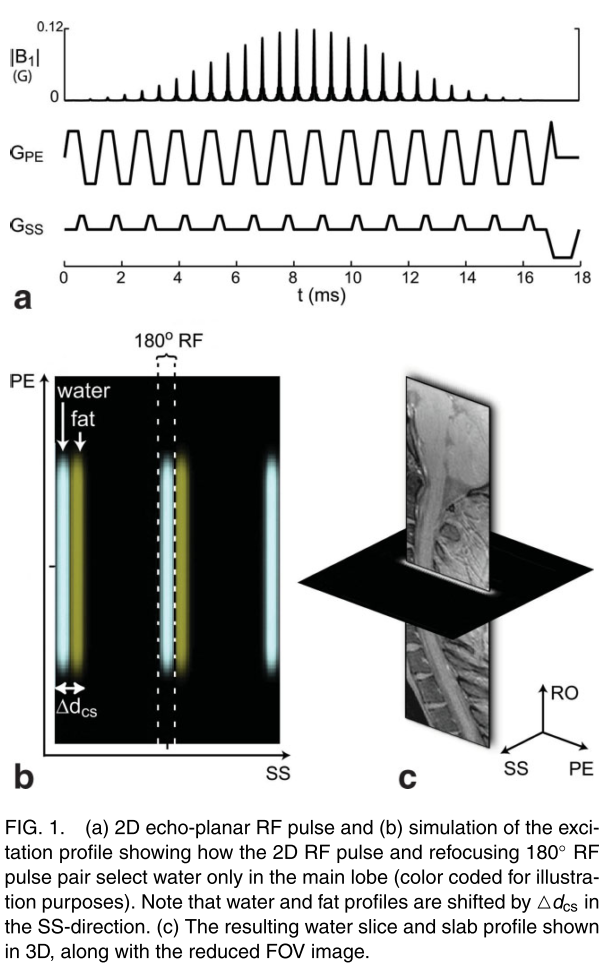
\includegraphics[height=6cm]{SpineDWIfig1}
	\end{column}
\end{columns}
\end{frame}

\begin{frame}{2D Echo-Planar RF Pulse}
\begin{columns}[T]
	\begin{column}[T]{5cm}
		\begin{itemize}
			\item The spatial displacement between fat and water caused by the echo-planar path of the 2D RF excitation pulse is $$\Delta d_{CS}=\frac{N_{blip}f_{CS}T_{fast}}{K_{blip}}$$
			\item The displacement $\Delta d_{CS}$ between fat and water can be designed so that the excited fat profile is entirely outside the water profile
		\end{itemize}
	\end{column}
	\begin{column}[T]{5cm}
		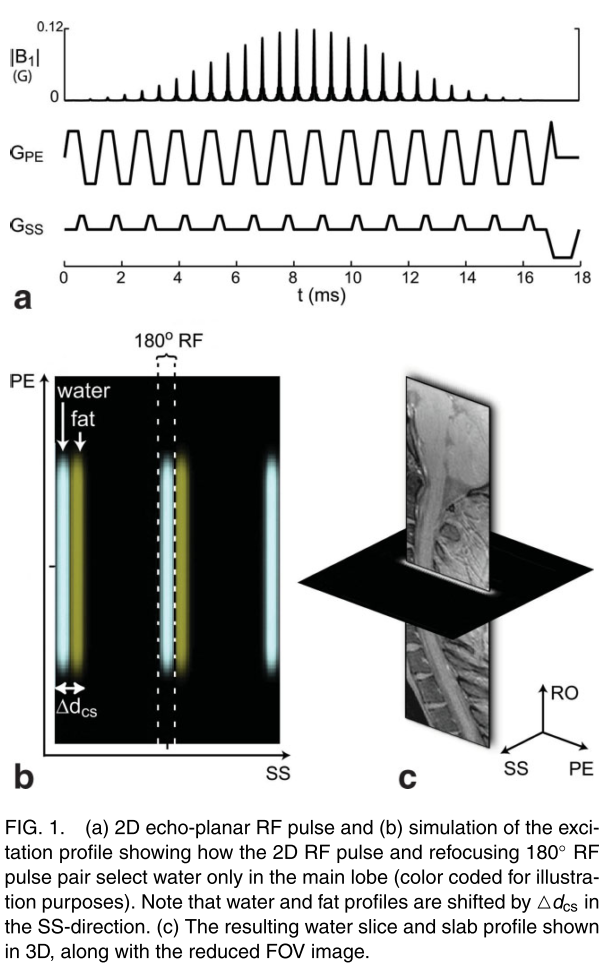
\includegraphics[height=6cm]{SpineDWIfig1}
	\end{column}
\end{columns}
\end{frame}

\begin{frame}{Refocusing RF Pulse}
\begin{itemize}
	\item After 2D RF excitation, a normal $180^{\circ}$ refocusing RF pulse is used, selective in SS direction
	\item Crusher gradients before and after the pulse are used
	\item Using 2D RF excitation pulse and $180^{\circ}$ refocusing RF pulse together suppresses signal from outside lobes of periodic 2D excitation and fat signal
	\item Fat suppression is particularly important in EPI, because fat signal can cause severe artifacts due to its dramatic shift in PE direction relative to water
\end{itemize}
\end{frame}

\subsection{Multi Slice Imaging}

\begin{frame}{Multi Slice Imaging}
\begin{itemize}
	\item Multi slice imaging is not possible for FOV restriction that uses two separate 1D RF pulses, which excites adjacent slices
	\item 2D echo-planar RF pulses do not excite adjacent slices, making contiguous multi slice imaging possible
	\item Upper limit on number of simultaneously imaged slices: $$max\left(N_{slices}\right)=\frac{\Delta d_{replicate}}{\Delta d_{SS}}=\frac{N_{blip}}{TBW_{SS}}$$
	\item With three sagittal slices the whole pulse sequence takes less than 120 ms per slice, allowing multi slice imaging in one cardiac cycle
\end{itemize}
\end{frame}

%%%%%%%%%%%%%%%%%%%%%%%%%%%%%%%%%%%%%%%%%%%%%%%%%%%%%%%%%%%%%%%%%%%%%%%%%%%
% Methods
%%%%%%%%%%%%%%%%%%%%%%%%%%%%%%%%%%%%%%%%%%%%%%%%%%%%%%%%%%%%%%%%%%%%%%%%%%%
%\section{Methods}
%\subsection{Phantom Experiments}
%\subsection{In Vivo Imaging}
%\subsection{Image Reconstruction}

%%%%%%%%%%%%%%%%%%%%%%%%%%%%%%%%%%%%%%%%%%%%%%%%%%%%%%%%%%%%%%%%%%%%%%%%%%%
% Results
%%%%%%%%%%%%%%%%%%%%%%%%%%%%%%%%%%%%%%%%%%%%%%%%%%%%%%%%%%%%%%%%%%%%%%%%%%%
\section{Results}
\subsection{Phantom Experiment Results}

\begin{frame}{Phantom Experiment Results}
	When using 2D selective RF pulse and $180^{\circ}$ refocusing pulse pair, no outer volume excitation is observed in phantom, and fat signal is suppressed
	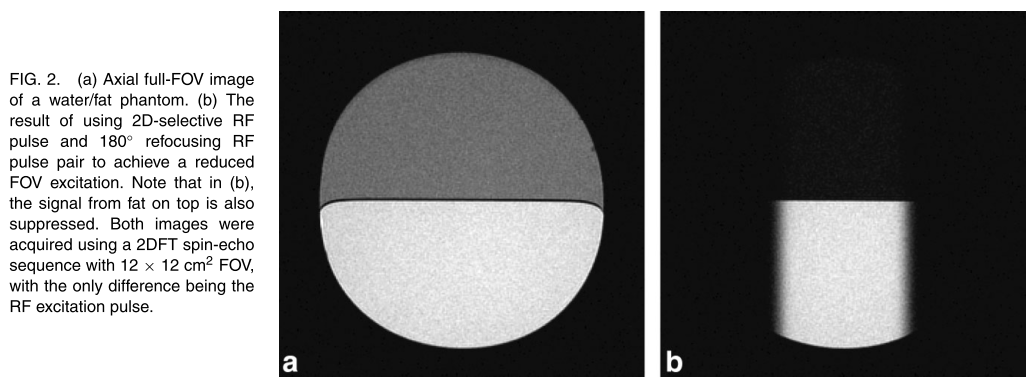
\includegraphics[height=4cm]{SpineDWIfig2}
\end{frame}

\subsection{In Vivo Imaging Results}

\begin{frame}{In Vivo Imaging Results}
\begin{columns}[T]
	\begin{column}[T]{5cm}
		\begin{itemize}
			\item Reduced FOV ss-EPI provides two times higher resolution for same readout time compared to full-FOV ss-EPI
			\item The trade-off is lower SNR due to four times smaller voxel size
		\end{itemize}
	\end{column}
	\begin{column}[T]{5cm}
		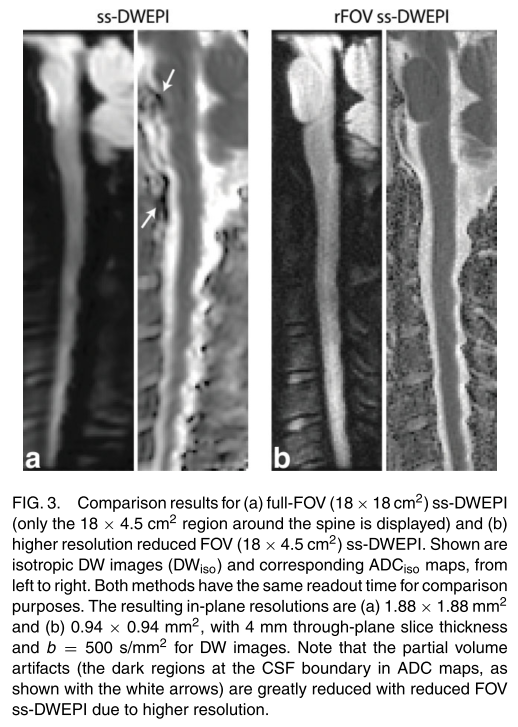
\includegraphics[height=6cm]{SpineDWIfig3}
	\end{column}
\end{columns}
\end{frame}

\begin{frame}{In Vivo Imaging Results}
	Non-DW, isotropic DW, and ADC maps for all three slices of the reduced FOV ss-EPI imaging
	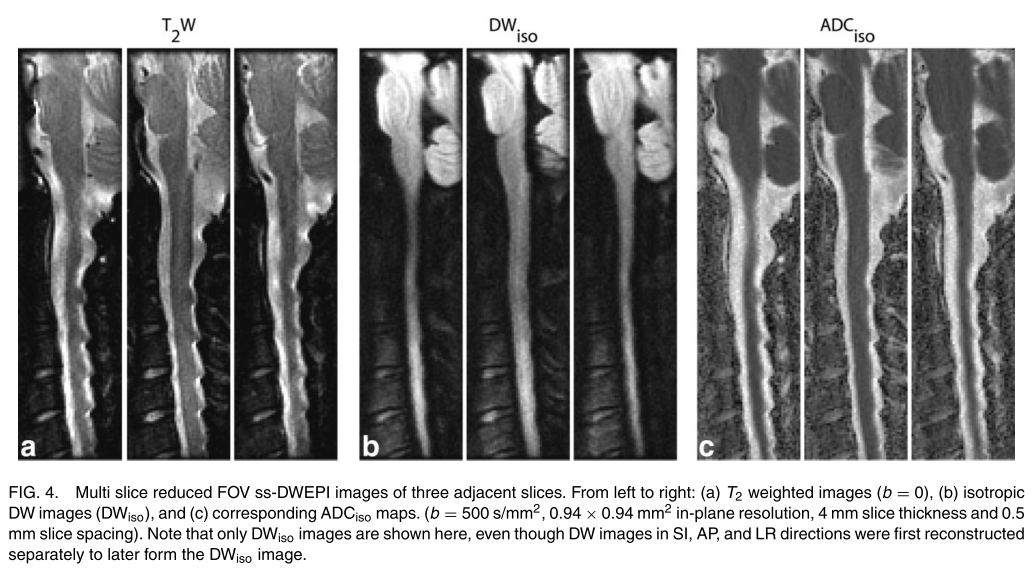
\includegraphics[height=6cm]{SpineDWIfig4}
\end{frame}

\begin{frame}{In Vivo Imaging Results}
\begin{columns}[T]
	\begin{column}[T]{5cm}
		\begin{itemize}
			\item Results of high-resolution axial DWI of cervical spinal cord with reduced FOV ss-EPI
			\item Demonstrate ability to acquire sub-mm DWI of spinal cord
		\end{itemize}
	\end{column}
	\begin{column}[T]{5cm}
		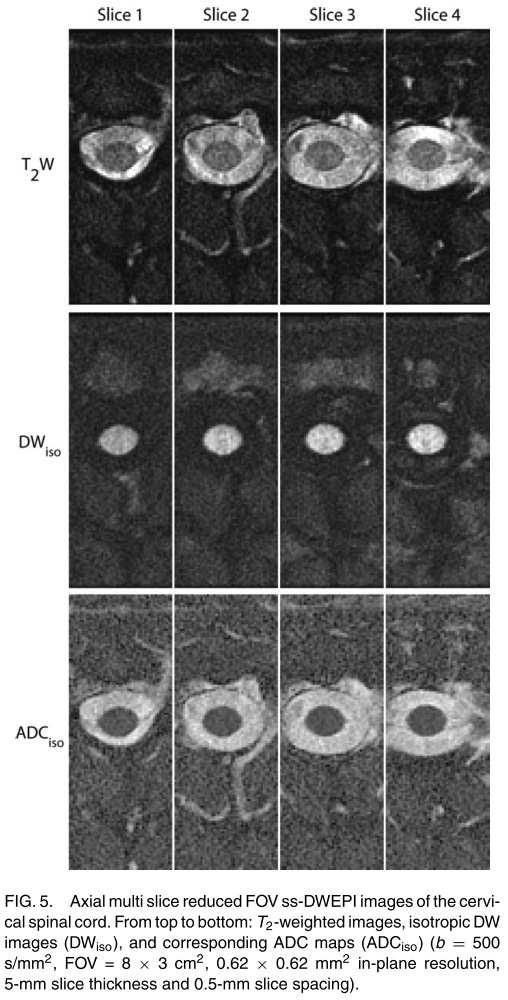
\includegraphics[height=6cm]{SpineDWIfig5}
	\end{column}
\end{columns}
\end{frame}

%%%%%%%%%%%%%%%%%%%%%%%%%%%%%%%%%%%%%%%%%%%%%%%%%%%%%%%%%%%%%%%%%%%%%%%%%%%
% Discussion
%%%%%%%%%%%%%%%%%%%%%%%%%%%%%%%%%%%%%%%%%%%%%%%%%%%%%%%%%%%%%%%%%%%%%%%%%%%
\section{Discussion}

\begin{frame}{Discussion}
\begin{itemize}
	\item Reduced FOV ss-EPI method excites minimum FOV to image ROI, reduces required k-space lines, and enables acquisition of higher resolution images for fixed scan time
	\item DW applied in three orthogonal directions reults in 10-minute scan time
	\item Can be extended to diffusion tensor imaging (DTI) for six or more directions and 15-20 minute scan time
	\item Compatibility with contiguous multi slice imaging is a significant advantage
\end{itemize}
\end{frame}

\begin{frame}{Discussion}
\begin{itemize}
	\item Fat suppression fails in certain regions due to bending in 2D echo-planar RF pulse only in non-axial images, because of large FOV in physical z-direction of scanner
	\item $B_0$ inhomogeneities become more pronounced with large FOV, resulting in bending of excitation profile when combined with long duration (16.8 ms) and concomitant fields from echo-planar gradients of 2D RF pulse
	\item Reduced FOV images with double resolution have quartered SNR
\end{itemize}
\end{frame}

%\subsection{Fat Suppression}
%
%\begin{frame}{Fat Suppression}
%\begin{itemize}
%	\item 
%\end{itemize}
%\end{frame}
%
%\subsection{Image Reconstruction}
%
%\begin{frame}{Image Reconstruction}
%\begin{itemize}
%	\item This technique is more robust than multi shot techniques, because no additional navigator echo is needed
%\end{itemize}
%\end{frame}

\end{document}

